\documentclass[a4paper]{article}
\usepackage{fullpage}
\usepackage{graphicx}

% Matlab Code Style Definition
\usepackage{listings}

\usepackage{color} %red, green, blue, yellow, cyan, magenta, black, white
\definecolor{mygreen}{RGB}{28,172,0} % color values Red, Green, Blue
\definecolor{mylilas}{RGB}{170,55,241}
\lstset{language=Matlab,%
    %basicstyle=\color{red},
    breaklines=true,%
    morekeywords={matlab2tikz},
    keywordstyle=\color{blue},%
    morekeywords=[2]{1}, keywordstyle=[2]{\color{black}},
    identifierstyle=\color{black},%
    stringstyle=\color{mylilas},
    commentstyle=\color{mygreen},%
    showstringspaces=false,%without this there will be a symbol in the places where there is a space
    numbers=left,%
    numberstyle={\tiny \color{black}},% size of the numbers
    numbersep=9pt, % this defines how far the numbers are from the text
    emph=[1]{for,end,break},emphstyle=[1]\color{red}, %some words to emphasise
    %emph=[2]{word1,word2}, emphstyle=[2]{style},    
}

\title{Simulated Annealing Hw5 ME 575}
\author{Ryan Day}
\date{\today}

\begin{document}
    \maketitle
    \section{Parameters, solution, and performance}
    \begin{center}
        \begin{tabular}{ |c |c |c |c | c| c| c| c| }
            \hline
          Starting Pt & Cycles & Iter/cycle & Pstart & Pfinish & Max Perturb & Fun Calls   \\ \hline
         5,5 & 10 & 6 & 1e-6 & 1e-30 & 4.5 & 60\\  \hline
        \end{tabular}
    \end{center}
    \subsection{Methodology}
    I implemented the simulated annealing algorithm in a function. 
    I then created a run routine that runs the simulated annealing algorithm with factorial combinations of parameters I choose.
    This run routine would run each combination 1000 times to reduce noise and count the number of times that combination found the optimum.
    My routine was fast enough that this did not put too big of a burden on the CPU.
    This helped me explore which parameters helped the simulated annealing algorithm converge the most.
    \subsection{Starting Points}
    I based my algorithm's performance on how it did from the edge points (5,5;-5,-5;-5,5;5,-5). 
    The edge points did the worst because they were most likely to perturb in a direction that was out of bounds, and so getting the algorithm to get out of the corner was a little slower than if I started more near the center.
    The points near the middle did better than the edge points in helping the algorithm to converge no matter what parameters I used.

    \subsection{Parameters}
    I chose parameters in the table above to minimize function calls and meet the around 7 out of 10 runs reaching the optimum that you provided us with. 
    The algorithm performs better with greater number of cycles and iterations per cycle because it has more chances to perturb the variables to the optimum and stay there.
    The next parameters were the probability starting and ending values. 
    These optimal parameters also depended on the step size.
    I chose a higher step size, 4.5. 
    Since we are searching a bounded box of 5 by 5 for an optimum, a step size of 4.5 with enough cycles and iterations practically guarantees that the algorithm will find the optimum eventually.
    This is because from any point, the algorithm can go to almost any other point.
    Since the optimum is in the middle, there was a very high chance the algorithm would find this optimum as the parameters were randomly perturbed.
    Because I used a high step size, it was actually better to have a very low Pstart and low Pfinish. 
    This prevents the algorithm from going uphill, but since the design space was so small, you know that it could always find the global optimum with enough iterations since with a step size of 4.5 the algorithm could reach practically anywhere in the design space from any other point.
    In this situation, the algorithm would go downhill by directly jumping to another minimum instead of following the curves of the contour plot.

    If the design space was much bigger with more variables with many more local minima, it would not be feasible to use the parameters that I did because it would be too computationally expensive.
    It would be better to have a higher Pstart, somewhere between 0.1 and 0.9 so that the algorithm wasn't relying on randomly finding the optimum with perturbations and instead was doing more valley descending and ascending.
    With higher dimensional space, it is not as simple to find optima.
    This is where the true power of simulated annealing lies. 
    It saves computational power, and is advantageous to a random search because it automatically gravitates towards large wells without getting stuck in a local minima.

    \subsection{Figures for a run with parameters in above table}
    \begin{center}
        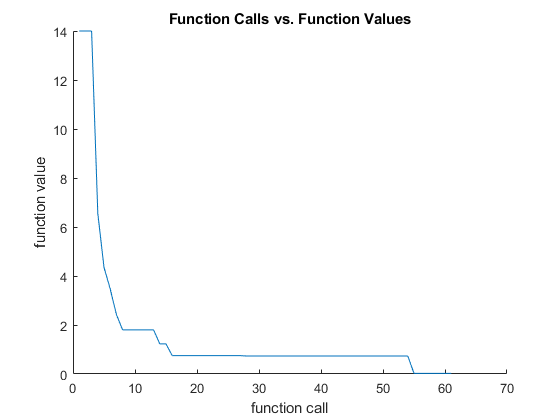
\includegraphics[scale = 0.7]{images/CallsVsValues.png}
        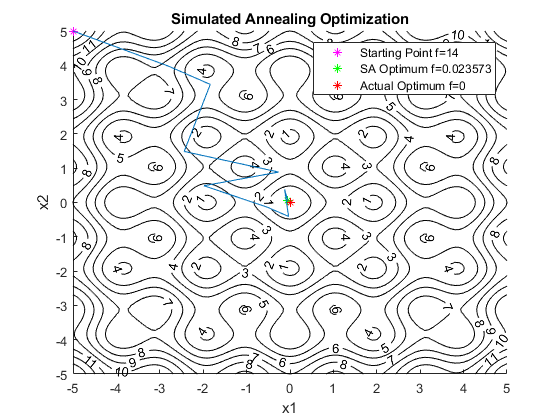
\includegraphics[scale = 0.7]{images/SimulatedAnnealingOptimization.png}
    \end{center}

    
    As you can see, because I gave it a very low Pstart, the algorithm never wandered around too much, staying at about 4 or 5 locations for all 60 perturbations. It would go directly to the next best optimum it found. 
    Like I said previously, while this works in a simple two dimensional problem, with a larger design space and a more complex non-linear function it would be better to have a higher P-start so that the algorithm doesn't get stuck in local optima.
    \section{Code}
    \subsection{Simulated Annealing algorithm with plotting and contour plots}
    \lstinputlisting{../simulatedAnnealing.m}
    \subsection{Simulated Annealing runner}
    \lstinputlisting{../runSimulatedAnnealing.m}
    
\end{document}